\documentclass[conference]{IEEEtran}

\IEEEoverridecommandlockouts

\usepackage[T2A]{fontenc}
\usepackage[utf8]{inputenc}
\usepackage[russian,english]{babel}
\usepackage{makecell}
\usepackage{multirow}

% The preceding line is only needed to identify funding in the first footnote. If that is unneeded, please comment it out.
\usepackage{amsmath,amssymb,amsfonts}
\usepackage{algorithmic}
\usepackage{graphicx}
\usepackage{textcomp}
\usepackage{multirow}
\usepackage{xcolor}
\usepackage[font=footnotesize]{caption}

\newif\ifblackandwhitecycle
\gdef\patternnumber{0}

\usepackage{tikz}
\usepackage{pgfplots}
\usetikzlibrary{spy,calc}
\newlength\imagewidth
\newlength\imagescale

\pgfkeys{/tikz/.cd,
	zoombox paths/.style={
		draw=orange,
		very thick
	},
	black and white/.is choice,
	black and white/.default=static,
	black and white/static/.style={ 
		draw=white,   
		zoombox paths/.append style={
			draw=white,
			postaction={
				draw=black,
				loosely dashed
			}
		}
	},
	black and white/static/.code={
		\gdef\patternnumber{1}
	},
	black and white/cycle/.code={
		\blackandwhitecycletrue
		\gdef\patternnumber{1}
	},
	black and white pattern/.is choice,
	black and white pattern/0/.style={},
	black and white pattern/1/.style={    
		draw=white,
		postaction={
			draw=black,
			dash pattern=on 2pt off 2pt
		}
	},
	black and white pattern/2/.style={    
		draw=white,
		postaction={
			draw=black,
			dash pattern=on 4pt off 4pt
		}
	},
	black and white pattern/3/.style={    
		draw=white,
		postaction={
			draw=black,
			dash pattern=on 4pt off 4pt on 1pt off 4pt
		}
	},
	black and white pattern/4/.style={    
		draw=white,
		postaction={
			draw=black,
			dash pattern=on 4pt off 2pt on 2 pt off 2pt on 2 pt off 2pt
		}
	},
	zoomboxarray inner gap/.initial=5pt,
	zoomboxarray columns/.initial=2,
	zoomboxarray rows/.initial=2,
	subfigurename/.initial={},
	figurename/.initial={zoombox},
	zoomboxarray/.style={
		execute at begin picture={
			\begin{scope}[
				spy using outlines={%
					zoombox paths,
					width=\imagewidth / \pgfkeysvalueof{/tikz/zoomboxarray columns} - (\pgfkeysvalueof{/tikz/zoomboxarray columns} - 1) / \pgfkeysvalueof{/tikz/zoomboxarray columns} * \pgfkeysvalueof{/tikz/zoomboxarray inner gap} -\pgflinewidth,
					height=\imageheight / \pgfkeysvalueof{/tikz/zoomboxarray rows} - (\pgfkeysvalueof{/tikz/zoomboxarray rows} - 1) / \pgfkeysvalueof{/tikz/zoomboxarray rows} * \pgfkeysvalueof{/tikz/zoomboxarray inner gap}-\pgflinewidth,
					magnification=3,
					every spy on node/.style={
						zoombox paths
					},
					every spy in node/.style={
						zoombox paths
					}
				}
				]
			},
			execute at end picture={
			\end{scope}
			\node at (image.north) [anchor=north,inner sep=0pt] {\subcaptionbox{\label{\pgfkeysvalueof{/tikz/figurename}-image}}{\phantomimage}};
			\node at (zoomboxes container.north) [anchor=north,inner sep=0pt] {\subcaptionbox{\label{\pgfkeysvalueof{/tikz/figurename}-zoom}}{\phantomimage}};
			\gdef\patternnumber{0}
		},
		spymargin/.initial=0.5em,
		zoomboxes xshift/.initial=1,
		zoomboxes right/.code=\pgfkeys{/tikz/zoomboxes xshift=1},
		zoomboxes left/.code=\pgfkeys{/tikz/zoomboxes xshift=-1},
		zoomboxes yshift/.initial=0,
		zoomboxes above/.code={
			\pgfkeys{/tikz/zoomboxes yshift=1},
			\pgfkeys{/tikz/zoomboxes xshift=0}
		},
		zoomboxes below/.code={
			\pgfkeys{/tikz/zoomboxes yshift=-1},
			\pgfkeys{/tikz/zoomboxes xshift=0}
		},
		caption margin/.initial=4ex,
	},
	adjust caption spacing/.code={},
	image container/.style={
		inner sep=0pt,
		at=(image.north),
		anchor=north,
		adjust caption spacing
	},
	zoomboxes container/.style={
		inner sep=0pt,
		at=(image.north),
		anchor=north,
		name=zoomboxes container,
		xshift=\pgfkeysvalueof{/tikz/zoomboxes xshift}*(\imagewidth+\pgfkeysvalueof{/tikz/spymargin}),
		yshift=\pgfkeysvalueof{/tikz/zoomboxes yshift}*(\imageheight+\pgfkeysvalueof{/tikz/spymargin}+\pgfkeysvalueof{/tikz/caption margin}),
		adjust caption spacing
	},
	calculate dimensions/.code={
		\pgfpointdiff{\pgfpointanchor{image}{south west} }{\pgfpointanchor{image}{north east} }
		\pgfgetlastxy{\imagewidth}{\imageheight}
		\global\let\imagewidth=\imagewidth
		\global\let\imageheight=\imageheight
		\gdef\columncount{1}
		\gdef\rowcount{1}
		\gdef\zoomboxcount{1}
	},
	image node/.style={
		inner sep=0pt,
		name=image,
		anchor=south west,
		append after command={
			[calculate dimensions]
			node [image container,subfigurename=\pgfkeysvalueof{/tikz/figurename}-image] {\phantomimage}
			node [zoomboxes container,subfigurename=\pgfkeysvalueof{/tikz/figurename}-zoom] {\phantomimage}
		}
	},
	color code/.style={
		zoombox paths/.append style={draw=#1}
	},
	connect zoomboxes/.style={
		spy connection path={\draw[draw=none,zoombox paths] (tikzspyonnode) -- (tikzspyinnode);}
	},
	help grid code/.code={
		\begin{scope}[
			x={(image.south east)},
			y={(image.north west)},
			font=\footnotesize,
			help lines,
			overlay
			]
			\foreach \x in {0,1,...,9} { 
				\draw(\x/10,0) -- (\x/10,1);
				\node [anchor=north] at (\x/10,0) {0.\x};
			}
			\foreach \y in {0,1,...,9} {
				\draw(0,\y/10) -- (1,\y/10);                        \node [anchor=east] at (0,\y/10) {0.\y};
			}
		\end{scope}    
	},
	help grid/.style={
		append after command={
			[help grid code]
		}
	},
}
\newcommand\phantomimage{%
	\phantom{%
		\rule{\imagewidth}{\imageheight}%
	}%
}
\newcommand\zoombox[2][]{
	\begin{scope}[zoombox paths]
		\pgfmathsetmacro\xpos{
			(\columncount-1)*(\imagewidth / \pgfkeysvalueof{/tikz/zoomboxarray columns} + \pgfkeysvalueof{/tikz/zoomboxarray inner gap} / \pgfkeysvalueof{/tikz/zoomboxarray columns} ) + \pgflinewidth
		}
		\pgfmathsetmacro\ypos{
			(\rowcount-1)*( \imageheight / \pgfkeysvalueof{/tikz/zoomboxarray rows} + \pgfkeysvalueof{/tikz/zoomboxarray inner gap} / \pgfkeysvalueof{/tikz/zoomboxarray rows} ) + 0.5*\pgflinewidth
		}
		\edef\dospy{\noexpand\spy [
			#1,
			zoombox paths/.append style={
				black and white pattern=\patternnumber
			},
			every spy on node/.append style={#1},
			x=\imagewidth,
			y=\imageheight
			] on (#2) in node [anchor=north west] at ($(zoomboxes container.north west)+(\xpos pt,-\ypos pt)$);}
		\dospy
		\pgfmathtruncatemacro\pgfmathresult{ifthenelse(\columncount==\pgfkeysvalueof{/tikz/zoomboxarray columns},\rowcount+1,\rowcount)}
		\global\let\rowcount=\pgfmathresult
		\pgfmathtruncatemacro\pgfmathresult{ifthenelse(\columncount==\pgfkeysvalueof{/tikz/zoomboxarray columns},1,\columncount+1)}
		\global\let\columncount=\pgfmathresult
		\ifblackandwhitecycle
		\pgfmathtruncatemacro{\newpatternnumber}{\patternnumber+1}
		\global\edef\patternnumber{\newpatternnumber}
		\fi
	\end{scope}
}

\usepackage[backend=biber, sorting=none]{biblatex}

% Symbols packages
\usepackage{ amssymb }

% Definitions of new commands
\newcommand{\bit}[1]{\ensuremath{\textbf{\textit{#1}}}}

%\bibliography{bibliography.bib}
\addbibresource{bibliography.bib}

\begin{document}

\title{Hardware optimized digital resamplers based on half-band filters\\
}
%\title{Hardware optimized half-band filters characteristics research\\
%}

\author{\IEEEauthorblockN{Bakholdin Nikita}
\IEEEauthorblockA{\textit{Moscow Power Engineering Institute (MPEI)} \\
\textit{National Research University}\\
Moscow, Russian Federation \\
bakholdin.nikita@gmail.com}
\and
\IEEEauthorblockN{Alexander Degtyarev}
\IEEEauthorblockA{\textit{Moscow Institute of Physics} \\
\textit{and Technology (MIPT)}\\
Moscow, Russian Federation \\
degtyarev.aa@phystech.edu}
\and
\IEEEauthorblockN{Sergey Bakhurin}
\IEEEauthorblockA{\textit{Moscow Power Engineering Institute (MPEI)} \\
\textit{National Research University}\\
Moscow, Russian Federation \\
bakhurinsa@mpei.ru}
}

\maketitle

	\begin{abstract}
		Current paper proposes the research of hardware optimized half-band filters exploitation as low-pass filters in a resampling scheme. Filters hardware optimization is implemented by the quantization algorithm, which allows to replace multipliers with the set of shift registers and adders. This approach provides reduction of a crystal area and power consumption. Also, current work proposes the research of the influence of hardware optimized filters difference from initial filters on the resampling scheme performance. In addition hardware complexity-reduced filters resources compared with the initial filters characteristics.
	\end{abstract}
	
	\section{Introduction}
	Digital resamplers are the class of digital devices that are used to change the sampling rate. This operations are common  in audio signal processing \cite{audio_resampler} and telecommunications \cite{resampler_telecom}.
	
	Digital signal processing structure that is shown on fig.~\ref{fig:resample_lpf} is widely used in synchronization tasks \cite{resample_sync} and in non-linear processing in order to decrease the influence of out-of-band components.
	
	Processing scheme is introduced on fig.~\ref{fig:resample_lpf}, where~$H(f)$,~$G(f)$ -- frequency responses of low pass filters,~$X(f)$,~$U(f)$,~$Q(f)$,~$Y(f)$ -- power spectral densities (PSD) of the input, upsampled, downsampled and output signals correspondingly. The scheme includes decimation and interpolation which imply discarding samples and zeros insertion correspondingly every~$L-1$ of~$L$ samples in the input signal. Also the scheme includes processing block~$P$ and low-pass filters ($LPF$) that are exploited in order to remove the replicated spectrum parts. 
	
	\begin{figure}[htbp]
		\centering
		\captionsetup{justification=centering}
		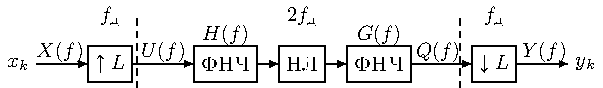
\includegraphics[scale=0.87]{Figures/resample_2_lpf+proc.pdf}
		\caption{Signal processing scheme with~$L$ times resampling}
		\label{fig:resample_lpf}
	\end{figure}
	
	LPF filters with finite impulse response (FIR) are widely used in digital resampling techniques \cite{dsp_oppenheim}. In case of rather high desired resampling factor~$L=2^M$, FIR filter must be of a high order, otherwise the whole resampler must be introduced by the~$M$-cascaded structure of low order low-pass filters and interpolators (decimators) with integer factor 2 \cite{lyons_multi_hbf}. 
	
	%It should be mentioned that in case of cascaded scheme optimal multistage resampling is achieved by different filter orders. Interpolator LPF orders must satisfy~$H > G > F$, where filters with orders~$H$,~$G$,~$F$ placed consistently, whereas decimators LPF orders must satisfy~$F > G > H$.
	
	Both filter order increase and cascaded structure implementation require hardware implementation of a high number of multipliers, which are the most complicated FIR-filters elements in terms of occupied crystal area and power consumption \cite{mults_complex}. More over, these parameters are growing quadratically depending on multipliers bit-depth \cite{mults_power_are_consum}.
	
	Therefore in order to reduce number of multipliers for resampler implementation without performance degradation half-band filters were suggested to use \cite{ch12_gockler}.
	
	The digital half-band filter (HBF) is, in its basic form with real-valued coefficients, a low-pass filter with passband and stopband regions of the same bandwidth.
	
	Real-valued HBF are widely used due to their properties such as symmetric impulse response and zero value of each 2-nd coefficient, which provide zero-valued phase response and efficient hardware implementation respectively~\cite{ch12_gockler}.
	
	Time-domain HBF impulse response~$h_k$ can be expressed in following way:
	\begin{gather*}
		h_k = h_{-k} =
		\begin{cases}
			1/2, & k=0, \\
			0, & k \ \text{mod} \ 2 =0, \\
			h_k, & k \ \text{mod} \ 2 =1.
		\end{cases}
	\end{gather*}
	
	Cutoff frequency of the HBF is defined as~$f_s/4$, where~$f_s$~is~a~sample rate.
	
	Due to their efficiency digital HBF are used as universal parts in applications for digital signal processing, in front ends of digital receivers and back ends of digital transmitters (software defined radio, modems etc. \cite{ren_multi_band}).
	
	However, despite the low computational load, required by the real-valued HBF, hardware implementation resources could be reduced even more with techniques represented in the next section. 
	
	\section{Resampling structures hardware implementation resources reduction}
	
	\subsection{Polyphase structure appoach}
	Calculation resources, required by processing scheme (fig.~\ref{fig:resample_lpf}) could be reduced with digital filter polyphase structure implementation \cite{vaidyanathan}.
	Such polyphase filter banks are useful in performing interpolation and decimation efficiently. 
	
	For instance, polyphase filter bank structure applied to the HBF provides~$50$\% multiplication per second reduction comparing to the direct filter implementation form. The examples of polyphase interpolator and decimator are shown on fig.~\ref{fig:polyphase_hbf_up},~\ref{fig:polyphase_hbf_down}.
	\begin{figure}[htbp]
		\centering
		\captionsetup{justification=centering}
		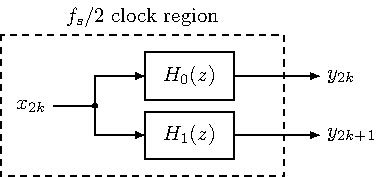
\includegraphics[width = 0.4\textwidth]{Figures/polyphase_upsampler.pdf}
		\caption{The upsampling operation by polyphase HBF}
		\label{fig:polyphase_hbf_up}
	\end{figure}
	\begin{figure}[htbp]
		\centering
		\captionsetup{justification=centering}
		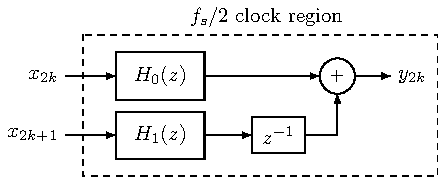
\includegraphics[width = 0.45\textwidth]{Figures/polyphase_downsampler.pdf}
		\caption{The downsampling operation by polyphase HBF}
		\label{fig:polyphase_hbf_down}
	\end{figure}
	where~$x_k$ -- input signal, samples~$y_{k}$~--~output signal,~$H_0(z)$,~$H_1(z)$ introduce transfer functions of polyphase subfilters with half number of multipliers. Note that filter with~$H_1(z)$ transfer function consist only of delay blocks and one non-zero central tap. This feature provides complexity-reduction in terms of multiplications per second due to~$H_0(z)$,~$H_1(z)$ work on~$f_s/2$ frequency.
	
	\subsection{Coefficients quantization approach}
	Another way to reduce half-band filter hardware implementation and calculation resources is to replace multipliers with bit shifters and adders, because signal division by 2 could be represented by the right 1 bit shift. Thus, the problem of multipliers replacement could be expressed as filter coefficients quantization, where each filter coefficient is expressed through other filter coefficients multiplied by the~$1/2^p$, where~$p\in\mathbb{N}_0$~\cite{fir_quant}.
	
	Denote coefficients of an arbitrary real-valued filter order~$N$ as~$\bit{h}\in\mathbb{R}^{N+1}$. Consider desired vector of coefficients~$\bit{b}\in\mathbb{R}^{M}$ -- basis coefficients, where~$M$ -- desired number of multipliers. As soon as initial vector of coefficients~$\bit{h}$ need to be described through the basis coefficients~$\bit{b}$, then desired coefficients are the subset of the initial coefficients~$\bit{b}\subset\bit{h}$.
	
	Reduced-complexity filter coefficient vector~$\bit{g}\in\mathbb{R}^{N+1}$ could be expressed through the transformation matrix~$\bit{T}\in~\mathbb{N}^{(N+1)\times M}$ and basis coefficient vector~$\bit{b}\in\mathbb{R}^{M}$ inner product \cite{fir_quant}:
	\begin{equation}
		\bit{g}=\bit{T}\bit{b}, \ \ \bit{T}=\{\textit{T}_{i,j}\}, \ \ i\in\overline{0,N},  \ \ j\in\overline{0,M-1},
		\label{reduced_filter_vector}
	\end{equation}
	As soon as initial coefficients are expressed through the basis coefficients multiplied by the powers of 2, then transformation matrix could be mathematically described in following way:
	\begin{equation}
		\textit{T}_{i,j}\in \{0, 2^{-p}\}, \ \ p\in \overline{0,K},
		\label{transform_matrix}
	\end{equation}
	where~$K$ -- fixed constant, that determines the precision of the quantization.
	
	Thus, the main point of the coefficients quantization approach is to find approximation vector~$\bit{g}$ to the initial coefficients~$\bit{h}$. This task could described as a search for the optimal pair of basis coefficient and power of 2 for each initial coefficient:
	\begin{equation}
		\begin{matrix}
			\forall i\in\overline{0,N}: \ p, j=\arg\min \left(\begin{vmatrix}\begin{vmatrix}h_{i}\end{vmatrix}-\begin{vmatrix}g_{j,p}\end{vmatrix}\end{vmatrix} \right), \\ \\
			g_{j,p}=\displaystyle{\frac{b_{j}}{2^{p}}}, \ j\in\overline{0,M-1}, \ p\in \overline{0,K}
		\end{matrix}
		\label{problem_formulation}
	\end{equation}
	Optimal pair~$\{b_j, 2^p\}$ for each~$h_i$ search algorithm in terms of \eqref{problem_formulation} is proposed in \cite{fir_quant}. 
	
	Coefficients quantization approach with search algorithm~\cite{fir_quant} are chosen for current paper as the HBF resources reduction method.
	
	\section{Half-band filters hardware optimization} \label{hbf_research}
	\subsection{Filters hardware optimization influence on the resampled signal}
	In current research the criteria of HBF hardware optimization is a number that corresponds to multiplications per second, which considered as~$\left \lceil{f_s(N+1)/4}\right \rceil$, where~$N$ -- filter order,~$\left \lceil{ \ \cdot \ }\right \rceil$ -- ceil operator. In case if hardware implemented processing does not include different clock regions, then optimization criteria is introduced by the number of HBF multipliers~$\left \lceil{(N+1)/4}\right \rceil$.
	
	As soon as reduced filter includes lower multipliers number comparing to the initial structure, then filter parameters such as transition bandwidth, level of stopband, passband lobes are changed. As a result input signal of the resampling scheme (fig.~\ref{fig:resample_lpf}) is processed with LPF, which parameters have been updated. Current section provides the research of multipliers number reduction influence on the signal processing quality.
	
	Test scheme is shown on fig.~\ref{fig:resample_lpf}. Resampling integer factor is chosen as~$L=2$. Considered HBF~$30$,~$62$ and~$94$ orders.
	\begin{figure}[htbp]
		\centering
		\captionsetup{justification=centering}
		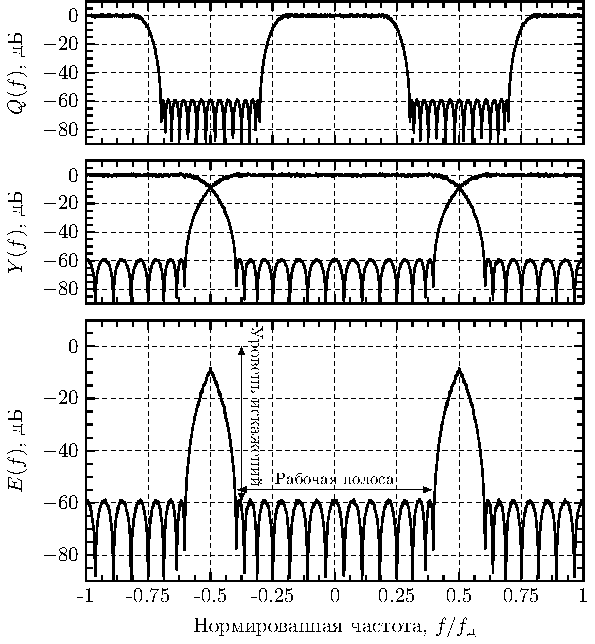
\includegraphics[width = 0.45\textwidth]{Figures/hbf_proc.pdf}
		\centering
%		\caption{White gaussian noise spectrum evolution in processing scheme with~$L=2$ times resampling}
		\caption{Преобразование спектра белого гауссовского шума в схеме передискретизации с~$L=2$}
		\label{fig:hbf_proc}
	\end{figure}
	
	White gaussian noise is chosen as a test input signal in resampling scheme (fig.~\ref{fig:resample_lpf}) due to it occupies whole spectral bandwidth, i.e. represents the most difficult case in terms of digital processing. 
	
	In following simulation scheme block~$P$ (fig.~\ref{fig:resample_lpf}) is assumed to be removed because the main point of current experiment is a research of resampler scheme influence on the input signal.
	
	Also, note that LPF frequency responses in current resampling scheme are considered to be the same~$H(f)=G(f)$.
	
	Figure~\ref{fig:hbf_proc} represents steps of signal processing in current experiment. Firstly, noise with power spectral density~$X(f)$ is upsampled resulting in signal with PSD~$U(f)$. Then, it propagates through two HBF, resulting power spectral density~--~$Q(f)$. Then filter output signal is downsampled with integer factor~$L=2$. As a result, spectrum copies overlap with the spectrum of neighboring Nyquist zones resulting in output signal with PSD~$Y(f)$ (fig.~\ref{fig:hbf_proc}). Finally, PSD~$E(f)$ represents the output signal spectrum and initial white noise spectrum difference~$E(f)$ -- PSD of difference $y_k-x_k$ . Thus, error PSD~$E(f)$ introduces resampling scheme influence on the input signal at the worst case in terms of signal bandwidth. 
	
	Note that error bandwidth of PSD~$E(f)$ (fig.~\ref{fig:hbf_proc}) shows the acceptable bandwidth of signal which could be processed in the resampling scheme (fig.~\ref{fig:resample_lpf}). Error level (fig.~\ref{fig:hbf_proc}) represents the level of distortion added to the signal with acceptable bandwidth after propagation through resampling scheme.
	
	\subsection{HBF quantization}	
	The aim of current paper is to research the dependence of the error level and error bandwidth (fig.~\ref{fig:hbf_proc}) on complexity-reduced filter multipliers number. Consider HBF with frequency response, shown on fig.~\ref{fig:filter_change}. Passband and stopband ripple levels could be tuned by changing transition bandwidth of the fixed-order filter. Transition bandwidth is adjusted by regulation of the parameter~$\alpha$ (fig.~\ref{fig:filter_change}), which is chosen from the discrete set of numbers. Thus, tuning parameter~$\alpha$ provides HBF with different passband and stopband ripple values. 
	
	\begin{figure}[htbp]
		\centering
		\captionsetup{justification=centering}
		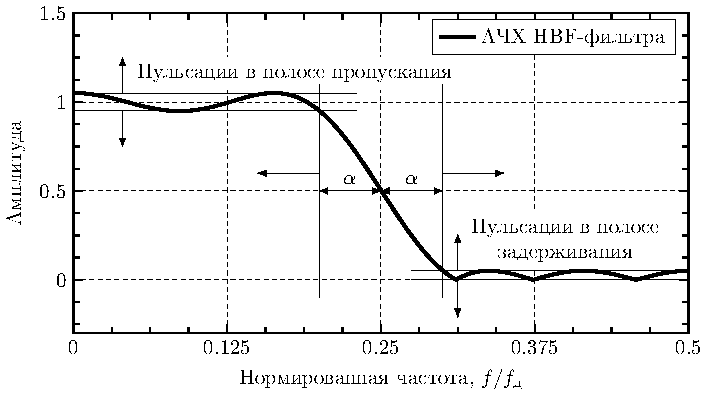
\includegraphics[width = 0.49\textwidth]{Figures/filter_change.pdf}
		\centering
%		\caption{Half-band low pass filter parameters tuning}
		\caption{Подстройка параметров фильтра половинной полосы}
		\label{fig:filter_change}
	\end{figure}

	Note that white gaussian noise error level (fig.~\ref{fig:hbf_proc}) is the sum of the passband ripple and spectrum copies stopband ripple. At the same time, stopband and passband ripples, as it was mentioned earlier, depend on the value of the transition bandwidth, which equals 2$\alpha$. As a result, in current experiment error level (fig.~\ref{fig:hbf_proc}) depends on the transition bandwidth.
	
	Error bandwidth also directly depends on the low pass filter transition bandwidth, which leads from fig.~\ref{fig:hbf_proc}. 
	
	Thus, error level and error bandwidth could be estimated for HBFs with different values of transition bandwidth, regulated by~$\alpha$-parameter.
	
	Consider HBFs order 30 synthesized for the discrete number of~$\alpha$-parameter (fig.~\ref{fig:filter_change}). In current experiment each of the mentioned filter is reduced in terms hardware resources by the algorithm~\cite{fir_quant}. Then, each of hardware-reduced filters is used as a low-pass filter in the resampling scheme (fig.~\ref{fig:resample_lpf}). Figure~\ref{fig:hbf32_full}~shows the error levels and error bandwidths of the input white gaussian noise after propagation through the resampling scheme with HBF with reduced multipliers number.
	
%	\begin{figure}[htbp]
%		\centering
%		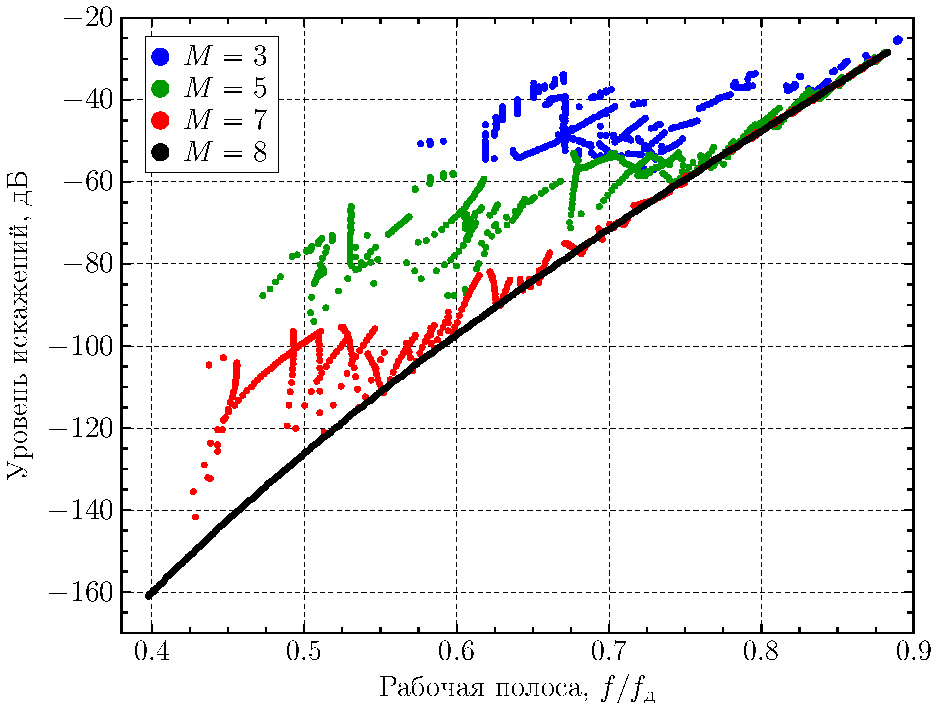
\includegraphics[width = 0.5\textwidth]{Figures/Points.pdf}
%		\caption{White gaussian noise error parameters after propagation through the downsampling scheme with complexity-reduced half-band low-pass filter}
%		\label{fig:hbf32_full}
%	\end{figure}
	\begin{figure}
		\centering
		\captionsetup{justification=centering}
		\pgfmathsetlength{\imagewidth}{\linewidth}%
		\pgfmathsetlength{\imagescale}{\imagewidth/524}%
		\begin{tikzpicture}[x=\imagescale,y=-\imagescale]
			\node[anchor=north west] at (0,0){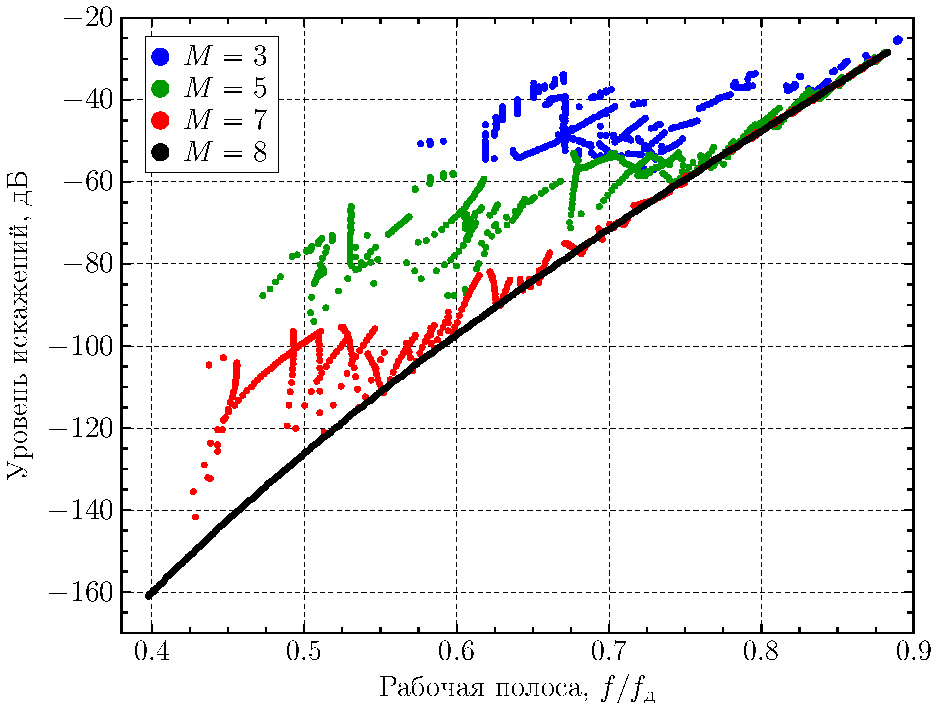
\includegraphics[width=\imagewidth]{Figures/Points.pdf}};
			\node[anchor=north west] at (260,195){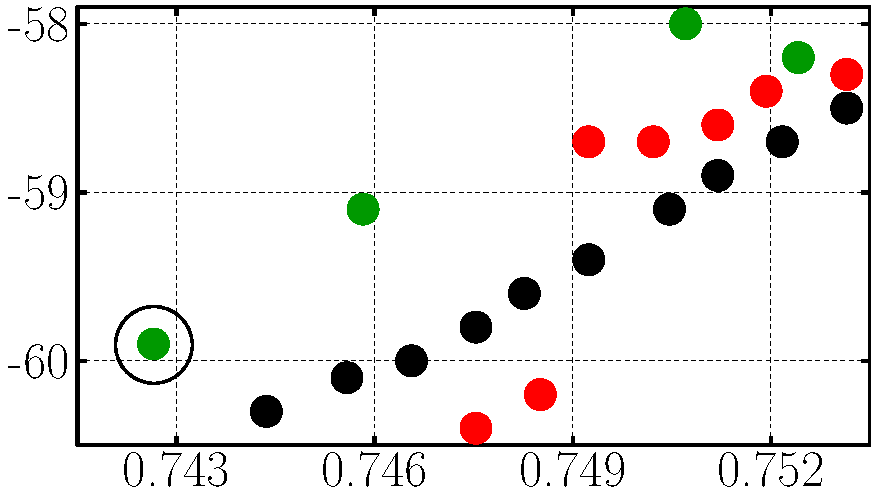
\includegraphics[ width=0.45\imagewidth]{Figures/Points_HBF32_part}};
			\node[draw, color = black, very thick, fill = none, minimum height=0.2cm,minimum width=0.4cm] at (385, 110) {};
		\end{tikzpicture}
%		\caption{White gaussian noise error parameters after propagation through the resampling scheme with complexity-reduced HBF.~$M$ -- multipliers number. The black rectangle represents the expanded area of the main figure}
		\caption{Параметры искажений вносимых схемой передискретизации с аппаратно оптимизированными фильтрами половинной полосы.~$M$ -- число умножителей. Чёрный прямоугольник указывает на область, представленную в увеличенном масштабе на основном рисунке.}
		\label{fig:hbf32_full}
	\end{figure}
	
	Multipliers number 8 is initial multipliers number of the HBF order 30 without quantization. It can be seen from fig.~\ref{fig:hbf32_full} that in case of using initial filter multipliers in resampling scheme~(fig.~\ref{fig:resample_lpf}), error level grows approximately linearly depending on the error bandwidth for the fixed filter order. Indeed, for the fixed filter order the lower transition bandwidth~$2\alpha$, the higher error bandwidth (fig.~\ref{fig:filter_change}), which means, higher passband and stopband ripples, that lead to higher error level (fig.~\ref{fig:hbf_proc}).
	
	On the other hand, fig.~\ref{fig:hbf32_full} shows that in case of reduced multipliers number the error level dependence on the error bandwidth is not even smooth, which occurs due to the quantization of the filter coefficients.
	
	The same evaluations obtained for the HBFs orders~62~and~94. Following section represents characteristics of mentioned complexity-reduced filters.
	
\section{Half-band filters complexity reduction examples}
Present section summarizes scheme error level, bandwidth and resources information for cases HBF 30, 62 and 94 orders (fig. \ref{fig:resample_lpf}). Filter parameters are chosen to satisfy the compromise between resampling scheme hardware implementation complexity and signal processing quality. In current paper~$-60$ dB error level is chosen as the resampling scheme quality criteria.

Consider HBF order 30 with the highest possible error bandwidth and error level, which not lower than~$-60$ dB. According to the expanded part of the fig.~\ref{fig:hbf32_full} such HBF includes 5 multipliers and~$0.743f_s$ error bandwidth. 

Filter hardware complexity is reduced by the algorithm~\cite{fir_quant}. Frequency response of the hardware optimized filter is shown on fig.~\ref{fig:hbf30_m5}.

\begin{figure}[htbp]
	\centering
	\captionsetup{justification=centering}
	
\includegraphics[width = 0.44\textwidth]{Figures/HBF_30_M5_FMR.pdf}
	\caption{Frequency response of the HBF order 30. $M$ -- filter multipliers number}
	\label{fig:hbf30_m5}
\end{figure}

PSD of the resampling scheme input~$X(f)$, output~$Y(f)$ (fig.~\ref{fig:resample_lpf}) and resampling scheme error~$E(f)$ are shown on fig.~\ref{fig:hbf62_m6}.

\begin{figure}[!h]
	\centering
	\captionsetup{justification=centering}
	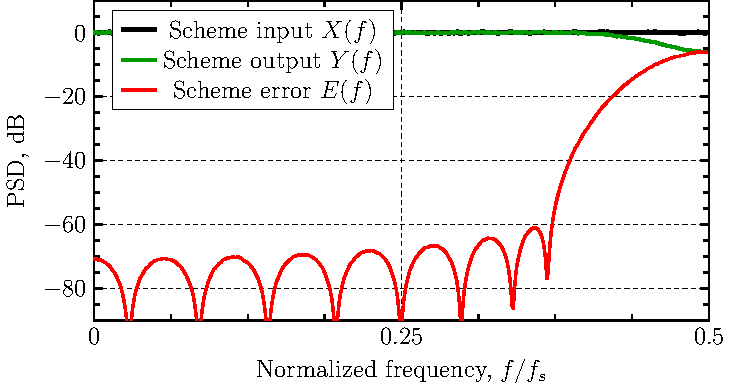
\includegraphics[width = 0.44\textwidth]{Figures/white_noise_filtering.pdf}
	\caption{Power spectral density of the resampling scheme input white gaussian noise, resampling scheme output and difference of input and output}
	\label{fig:hbf62_m6}
\end{figure}

Table~\ref{tbl:article_summary} summarizes information of complexity-reduced filters resources, acquired by quantization algorithm \cite{fir_quant}, represents the comparison with initial reference filters and compares resources and scheme quality with filters with the same order and approximately the same error level. 

The table~\ref{tbl:article_summary} shows that for filter order 30 error bandwidth and error level remained approximately the same, but hardware multiplications~$40\%$ reduced.

In case of HBF order 62 resampling scheme with optimized filter error level is about~$-60$ dB, while the initial filter provides~$-100$ dB. Error bandwidth is~$5\%$ lower comparing with filter of the same order, which provides the same error level. But, hardware implementation complexity reduction is around~$63\%$ comparing to non-simplified filters.

For the case of HBF order 94 resampling scheme with optimized filter error level is approximately~$-60$ dB, whereas the initial filter corresponds to~$-140$ dB. Error bandwidth is~$12\%$ in comparison with the same order and the same error level filter. Complexity reduction is around~$70\%$ comparing to the non-optimized filters.

The structure of complexity reduced HBF order 30 with 5 multipliers is shown on fig.~\ref{fig:hbf30_str}.

\begin{table}[hbtp]
%	\caption{Resource estimation table for complexity reduced HBF filters}
	\caption{Оценка ресурсов аппаратно оптимизированных фильтров половинной полосы}
	%\begin{center}
	\centering
	\resizebox{0.5\textwidth}{!}{%
		\begin{tabular}{|c|c|c|c|c|c|}
			\hline
			\makecell{Порядок \\ фильтра} 
			& \makecell{Число \\ умножителей}  
			& \makecell{Число \\ сумматоров}   
			& \makecell{Число сдвиговых \\ регистров}   
			& \makecell{Уровень \\ искажений, дБ}   
			& \begin{tabular}[c]{@{}c@{}} 
				Рабочая полоса \\ 
				для $-60$ дБ, ~$f/f_{\text{д}}$ 
			\end{tabular} \\ \hline
			
			\multirow{2}{*}{N = 30}       & 5           & \begin{tabular}[c]{@{}c@{}}11 (2 порт)\\ или\\ 2 (6 порт)\\ 1 (4 порт)\\ 3 (2 порт)\end{tabular}                                         & 7       & -60  & 0.743  \\ \cline{2-6}    & 8 & \begin{tabular}[c]{@{}c@{}} 1 (9 порт) \\ 8 (2 порт) \end{tabular}  & 1 & -61 & 0.745 \\ \hline
			
			\multirow{2}{*}{N = 62}       & 6           & \begin{tabular}[c]{@{}c@{}}26 (2 порт)\\ или\\ 2 (8 порт)\\ 1 (7 порт)\\ 3 (4 порт)\\ 1 (3 порт)\\ 1 (2 порт)\end{tabular}               & 21    & -61  & 0.817  \\ \cline{2-6}    & 16 & \begin{tabular}[c]{@{}c@{}} 1 (9 порт) \\ 16 (2 порт) \end{tabular} & 1 & -100 & 0.812 \\ \cline{2-6}    & 16 & \begin{tabular}[c]{@{}c@{}} 1 (9 порт) \\ 16 (2 порт) \end{tabular} & 1 & -62 & 0.868 \\\hline
			
			\multirow{2}{*}{N = 94 }      & 7           & \begin{tabular}[c]{@{}c@{}}41 (2 порт)\\ или\\ 1 (18 порт)\\ 2 (8 порт)\\ 2 (6 порт)\\ 1 (4 порт)\\ 1 (3 порт)\\ 2 (2 порт)\end{tabular} & 35    & -62  & 0.810  \\ \cline{2-6}    & 24 & \begin{tabular}[c]{@{}c@{}} 1 (25 порт) \\ 24 (2 порт) \end{tabular} & 1 & -140 & 0.804 \\ \cline{2-6}    & 24 & \begin{tabular}[c]{@{}c@{}} 1 (25 порт) \\ 24 (2 порт) \end{tabular} & 1 & -62.2 & 0.911 \\\hline
		\end{tabular}%
	}
	%\end{center}
	\label{tbl:article_summary}
\end{table}

\section*{Conclusions}
Current work researches the influence of the filter optimization on resampling scheme performance and compares hardware optimized filters with non-optimized filters of the same order that provide the same scheme quality.

Quantization algorithm provides up to~$40\%$,~$63\%$ and~$70\%$ multiplications per second reduction for half-band filters order 30, 62 and 94 correspondingly.

Acceptable bandwidth for signal processing in scheme with optimized filters is about~$0.5\%$,~$5\%$ and~$12\%$ lower for filters order~$30$,~$62$ and~$94$ correspondingly comparing to the non-optimized filters of the same order, which provide the same resampling scheme output deviation from the input, approximately equal~$-60$ dB.

\begin{figure*}[!h]
	\captionsetup{justification=centering}
	\centering{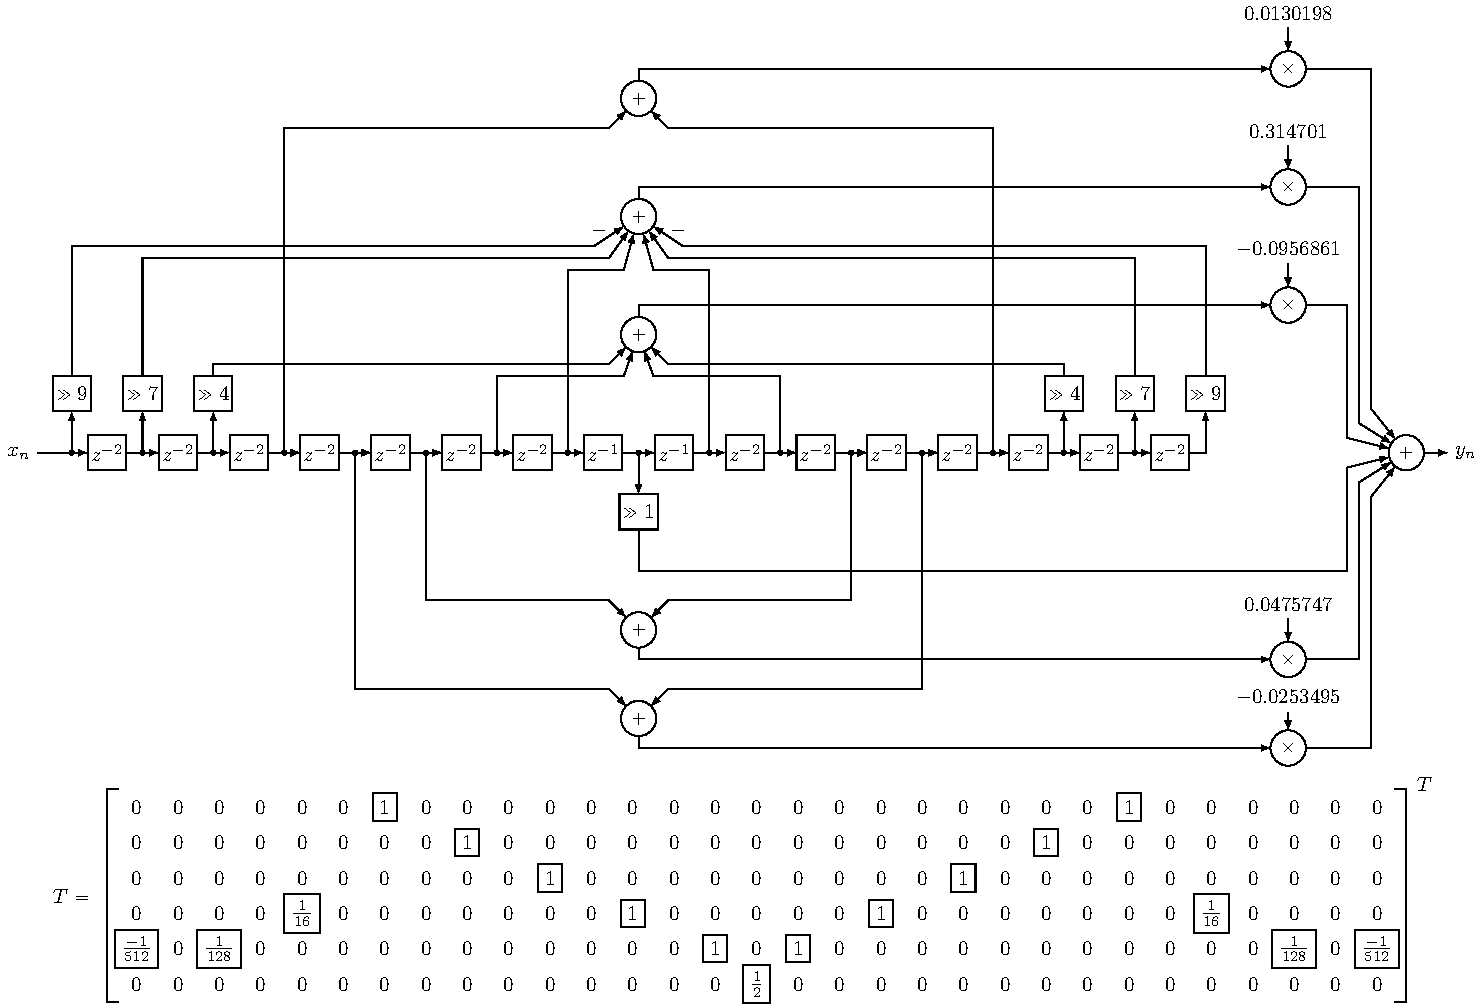
\includegraphics[width=0.99\linewidth]{Figures/hbf_structure.pdf}}
    \caption{HBF order 30 structure and transposed transformation matrix of quantization algorithm}
    \label{fig:hbf30_str}
\end{figure*}

%\clearpage
\printbibliography

%\printreference

\end{document}